\section{Visual Inspection}
Visual inspection is a primary, non-destructive method 
for evaluating the integrity of optical contact bonds. 
The physical principle underlying this technique is 
thin-film interference, which manifests visibly as Newton's 
rings when the contacting surfaces are illuminated. 
\\\\
In an ideal optical contact bonding process, the interfacial 
air gap is completely eliminated. Optically, this results in 
the disappearance of interference fringes, indicating a defect-free 
and continuous bond. However, the presence of Newton's rings during or after the 
bonding process serves as a direct indicator of interfacial 
defects. 
These interference patterns occur due to localized 
variations in the gap thickness between the two surfaces.
Issues can be identified and evaluated through this phenomenon are
trapped air and voids, particulate contamination and surface flatness
deviations \cite{pasternak2018,rammhandbook}. 
Figure \ref{fig:newtonrings} shows an example of 
Newton rings.
\\\\
Depending on the optical properties of the materials involved, visual 
inspection is conducted using different setups. For transparent optical 
components, monochromatic or white light interferometry is typically 
used. Conversely, for materials that are opaque in the visible spectrum, 
such as silicon wafers, infrared (IR) transmission imaging is 
routinely employed to visualize these interference patterns at the 
bonding interface \cite{masteika2014}. Ultimately, an interfacial region completely devoid 
of visible Newton's rings serves as the standard criterion for a successful, 
defect-free optical contact bond.
\begin{figure}[h]
    \centering
    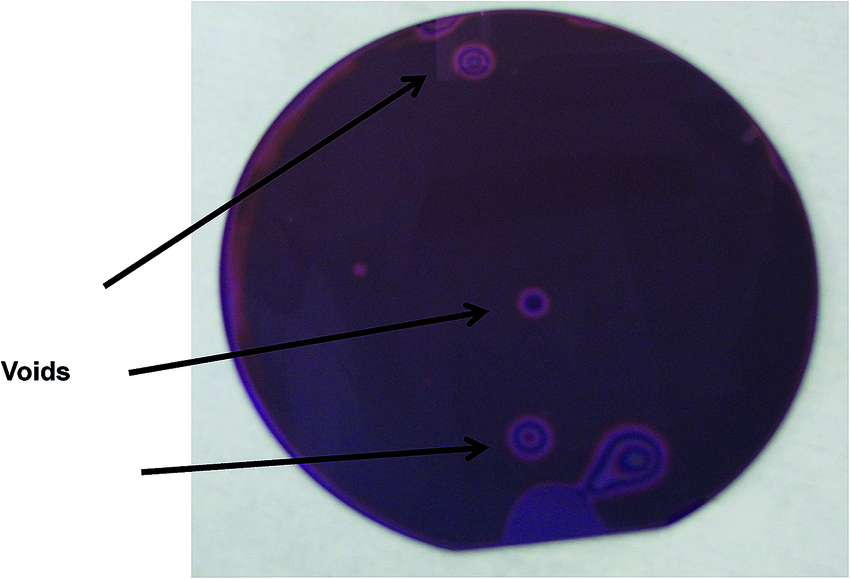
\includegraphics[width=0.8\linewidth]{Images/newtonrings.png}
    \caption{Newton rings being formed on the interfase
    of a SiN-glass wafer. From \cite{pasternak2018}.}
    \label{fig:newtonrings}
\end{figure}
